\section{Data}
Data is units of information, and in a technical perspective, data is a set
of values of quantitative or qualitative variables about a data object. 
Data should be understood in the context of information. Information can be 
thought of as the resolution of uncertainty, though it's 
exact interpretation and meaning differs in different context. Using this
vague definition of information it becomes clear how diverse data can be.
Everything that removes uncertainty contains information and can potentially 
be stored and processed as data. Examples of data can be 

\begin{itemize}
    \item Tabular Data like spreadsheets.
    \item A news article.
    \item A photograph.
    \item A TV broadcast.
    \item And much much more.
\end{itemize}

Historically, computation has been done on numerical data like tabulated data,
but in the later decades data mining and machine learning methods have broadened
what data algorithms can use to do inference. One example is Neural Networks
and image classification.

\section{Data Mining}
Data mining can be described as:

\begin{center}
    \textit{"Non-trivial extraction of implicit, \\
    previously unknown and potential useful information from data"}
\end{center}

\begin{center}
    \textit{"Exploration and analysis, by automatic or semi-automatic means, \\
    of large quantities of data in order to discover meaningful patterns"}
\end{center}

Data mining is a process of extracting 
and discovering patterns in large data sets involving methods at the 
intersection of machine learning, statistics, and database systems. 
Data mining is an interdisciplinary subfield of computer science and statistics 
with an overall goal to extract information (with intelligent methods) 
from a data set and transform the information into a comprehensible structure 
for further use. \cite{enwiki:datamining}

\section{Machine Learning}

Machine learning can be described as:

\begin{center}
    \textit{"The field of study that gives computers the ability to learn \\
    without being explicitly programmed"}
\end{center}

\begin{center}
    \textit{"A computer program is said to learn from experience E \\
     with respect to some class of tasks T and performance measure P, \\
     if its performance at tasks in T, as measured by P, improves with experience E"}
\end{center}

\newpage
\section{Data Mining or Machine Learning}

Data mining is the process of discovering patterns in large data sets involving methods at the interseciton of machine learning, statistics, and database systems.
\begin{figure}[H]
    \centering
    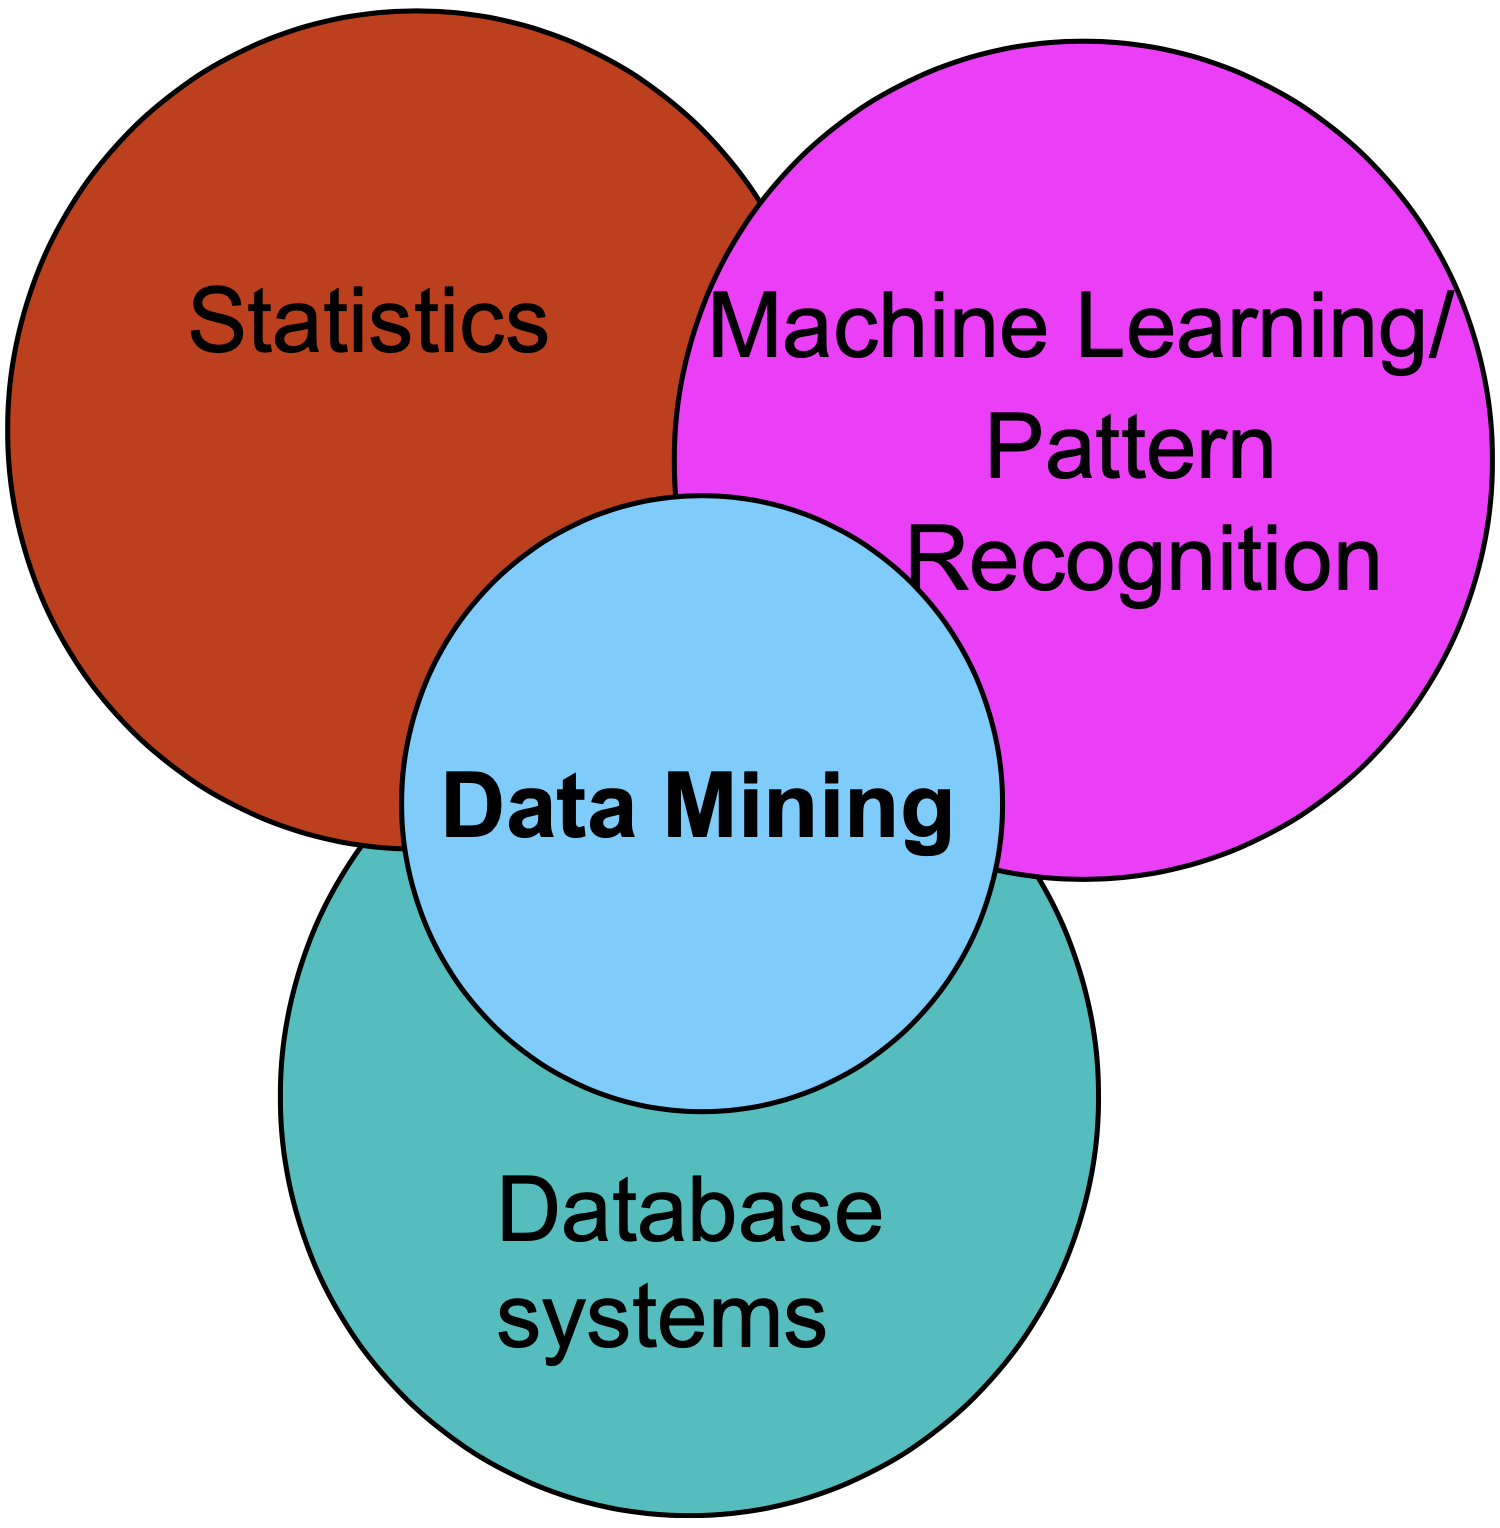
\includegraphics[scale=0.2]{figures/datamining.png}
    \caption{Diagram of Data Mining}
\end{figure}


\section{Properties of Data Mining}
\subsection{Commercial viewpoint}
Lots of data is being collected and warehoused, such as web data, purchases, and transactions.
Computation power has become cheap and powerful, and the competitive pressure is strong.
It is therefore necessary to provide better, customized servicees for an edge.

\subsection{Scientific Viewpoint}
Data is collected and stored at enormous speeds, up to multiple terrabytes per hour.
Such data can be generated from the large hydron collider and from scanning the universe.
Such data can not be interpreted by traditional techniques, and requires data mining to classify and segment the data,
and form hypothesis formations.

\newpage
\subsection{KDD Process}
Knowledge Discovery in Databases (KDD) refers to the overall process of discovering useful knowledge from data.

KDD is an integration of multiple technologies for data management such as database management and data warehousing, 
statistic machine learning, decision support, and others such as visualisation and parallel computing. 

\begin{figure}[H]
    \centering
    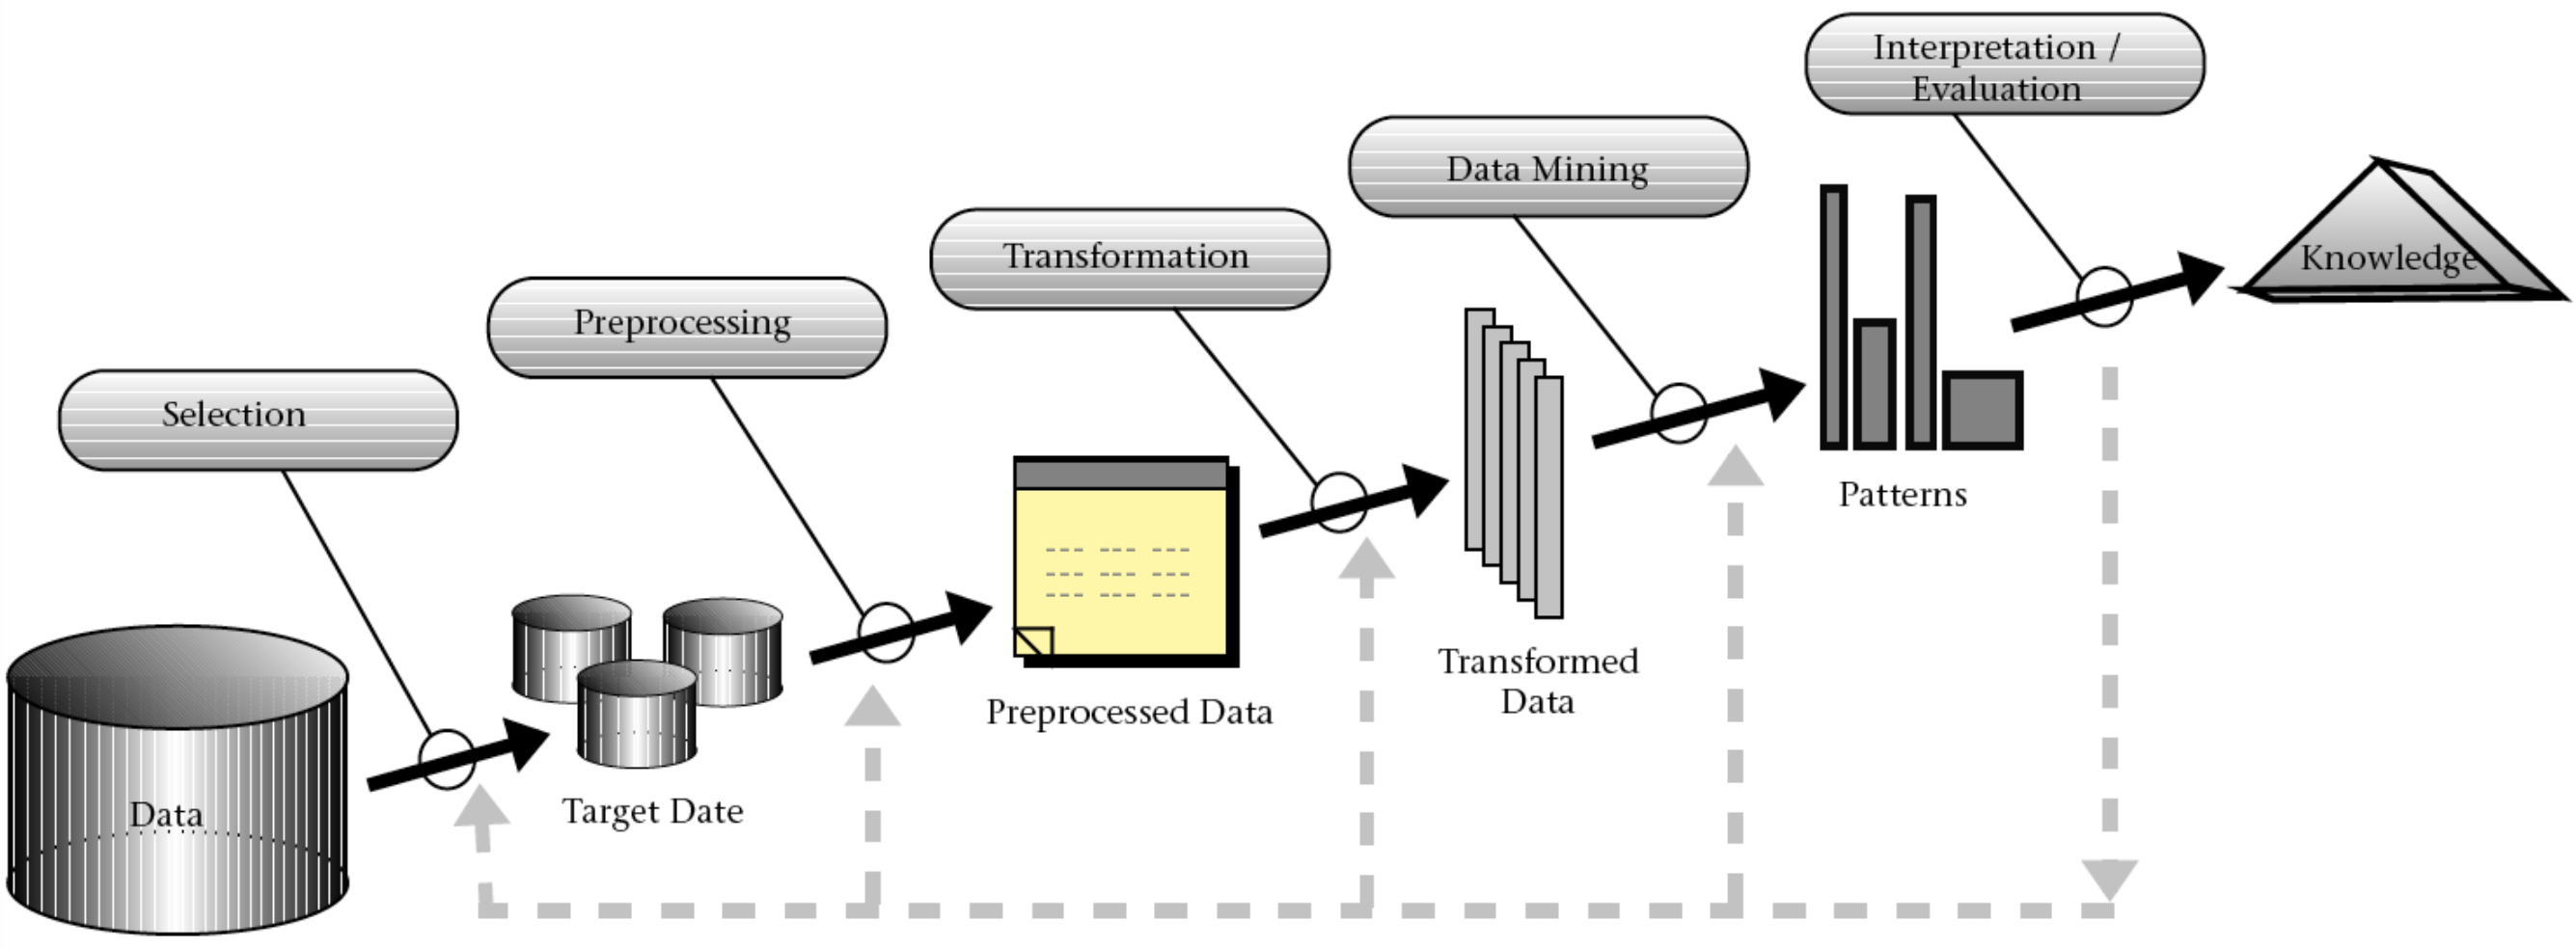
\includegraphics[scale=0.2]{figures/kdd.png}
    \caption{The KDD Process}
\end{figure}

\section{Data Mining tasks}
\begin{itemize}
    \item Prediction methods
    \begin{itemize}
        \item Use some variables to predict unknown or future values of other variables.
        \begin{itemize}
            \item Supervised (classification or regression)
            \item Unsupervised (clustering)
            \item Semi-supervised
        \end{itemize}
    \end{itemize}
    \item Descriptive methods
    \begin{itemize}
        \item Find human-interpretable patterns that describe the data.
        \begin{itemize}
            \item Rule mining
            \item Frequent patterns
            \item Anomaly detection
        \end{itemize}
    \end{itemize}
\end{itemize}

\section{Regression}
\begin{enumerate}
    \item Given a set of data points/instances along with “correct” answers or 
    labels (training data)
    \item Feed it to an algorithm which can learn a model and predict the 
    correct value for an unseen data point (test data)
    \item The learned model is an approximate representation of the training 
    data
    \item Predict continuous valued output (price in the previous example)
    \item The algorithm should produce more right answers (goal)
\end{enumerate}

\section{Unsupervised Learning}
\begin{itemize}
    \item Unsupervised learning includes unlabeled data
    \item One way of doing this would be to cluster data into to groups
    \begin{itemize}
        \item Group data points which are similar together, while separating 
        dissimilar items as much as possible
        \item This is a clustering algorithm
    \end{itemize}
\end{itemize}

\section{Association Rule Mining}
\begin{itemize}
    \item Given a set of records each of which contain some number of items from a given collection
    \item Produce dependency rules which will predict occurrence of an item based on occurrences of other items
\end{itemize}
Such rules can be used for marketing and sales promotion. Rule mining can also be used for inventory management, and much more.

\section{Challenges in Data Mining}
\begin{itemize}
    \item Scalability
    \item Dimensionality
    \item Heterogenous or complex data
    \item Data ownership and distribution
    \item Privacy concern
    \item Data quality
    \item Evolving/streaming data
\end{itemize}

